%______________________________________________________________________________________________________________________
% @brief    LaTeX2e Resume
%\documentclass[article]{resume}
\documentclass{article}
\usepackage[legalpaper, top=0.5in, left=0.4in, bottom=0.5in, right=0.6in]{geometry}
\usepackage{graphicx}
\usepackage{ragged2e}
\usepackage{url}
\usepackage{amsmath}
\usepackage{amssymb}
\usepackage{titlesec}

\usepackage[scaled]{helvet}
\renewcommand\familydefault{\sfdefault} 
\usepackage[T1]{fontenc}
\usepackage{multicol}
\urlstyle{same}
\frenchspacing
\graphicspath{{./images/}}
\usepackage{enumitem}

\titleformat{\section}[block]
{\Large\bfseries}
{\thesection.}{0.5em}{}
 
\titlespacing{\section}{-12px}{6px}{6px}

%______________________________________________________________________________________________________________________
\begin{document}
%\fontfamily{lmr}\selectfont  - font
{

%
\begin{minipage}[t]{0.33\textwidth}
\begin{flushleft}
 \textbf{\large{Devin Bonnie}}
 \vspace{4px}
\linebreak
\small{Realizing a passion for the environment by providing realiable platform capabilities through ocean robots. Experience in operational robotics, software design, computer vision, and embedded systems. Aiming to describe behavior empirically.\\}
\vspace*{1\baselineskip}
\end{flushleft}
\end{minipage}	
\begin{minipage}[c]{0.33\textwidth}
\begin{center}
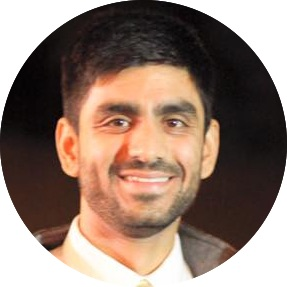
\includegraphics[trim= 0cm 10cm 0 0cm,scale=0.22]{dbCircle}
\end{center}
\end{minipage}
\begin{minipage}[t]{0.33\textwidth}
\begin{flushright}
\vspace*{1\baselineskip}
devin.bonnie@gmail.com
 \vspace{2px}
\linebreak
(810) 623-2687
 \vspace{2px}
\linebreak
Sunnyvale, CA 
 \vspace{2px}
\linebreak
https://github.com/wriggityWrecked
\linebreak
\end{flushright}
\end{minipage}
%
\linebreak
\rule{560px}{0.25pt}

\setlength{\columnsep}{30px}
\begin{multicols}{2}

%
%
%%__________________________________________________________________________________________________________________
    % Education
\section*{Education}
\noindent
\textbf{University of Illinois at Urbana-Champaign}, Illinois\\
\textsl{M.S., Electrical and Computer Engineering}\\
\textsl{2011}\\
\textsl{Advisor:} S.A. Hutchinson \hfill\\
\linebreak
%\vspace{2px}
\noindent
\textbf{Hope College}, Michigan\\
\textsl{B.S., Engineering (Electrical Emphasis), Mathematics Minor} \hfill\\
\textsl{2007}
\vspace{-4px}
    \begin{itemize}
        \item[\tiny$\bullet$]Senior project recognized with the \textit{VanPutten Engineering Design Award}.
    \end{itemize}
    \vspace{ -2 mm}
    %__________________________________________________________________________________________________________________
    % Experience
\section*{Experience}
\noindent
    \textbf{Liquid Robotics, A Boeing Company}\\
    Staff Software Engineer\\
    Technical Lead \hfill \textsl{June 2017 -- Present} \\
    \vspace{ -10px}
    \begin{itemize}[noitemsep,nolistsep]
        \item[\tiny$\bullet$ ]Architected various components including naviagtional control, communications protocols, and a vehicle \\ simulation environment.
    \end{itemize}
    \vspace{5px}
    \textbf{Liquid Robotics}\\
    Senior Software Engineer\\
    Technical Lead \hfill \textsl{May 2014 -- June 2017} \\
    \vspace{ -10px}
    \begin{itemize}[noitemsep,nolistsep]
         \item[\tiny$\bullet$] Lead as vehicle operating system technical lead before and during Boeing acquisition.
         \item[\tiny$\bullet$] Operations support lead, routinely diagnosed and applied root cause analysis to customer-facing issues.
         \item[\tiny$\bullet$] Implemented live hurricane-tweeting drone that generated national news.
    \end{itemize}
    \vspace{5px}

    \textbf{Payload Software and Vehicle Software} \hfill Software Engineer\\  
    Liquid Robotics \hfill \textsl{Aug. 2012 -- Apr. 2014} \\
    \vspace{ -2 mm}
    \begin{itemize}
        \item Vehicle control system contributions included work on navigation, communications, and sensors.
        \item Integrated multiple sensors for SV2 and SV3 platforms, e.g., cameras, GPS, weather, oceanographic.
    \end{itemize}\vspace{-2mm}

    \textbf{ISDA Group} \hfill Research Programmer\\  
    National Center for Supercomputing Applications \hfill \textsl{Oct. 2011 -- Jul. 2012} \\
    \vspace{ -2 mm}
    \begin{itemize}
        \item Responsibilities included image comparison techniques, data visualization, and automated decision support. 
        \item Other tasks included efficient incorporation/rendering of 3D image data over lossy network streams.  
    \end{itemize}\vspace{-2mm}
   
    \textbf{Software Technology Group} \hfill Intern\\  
    Wolfram Research, Inc. \hfill \textsl{Summer 2011} \\
    \vspace{ -2 mm}
    \begin{itemize}
        \item Contributed to a developmental C++ robotics API for both specification and implementation.
	 \item Accomplished reliable communication, file I/O, and robust sensor measurement methods. 
    \end{itemize}\vspace{-2mm}

    \textbf{Dept. of Electrical and Computer Engineering} \hfill Teaching Assistant/Research Assistant \\  
    University of Illinois at Urbana-Champaign \hfill \textsl{Jan. 2010 -- Aug. 2011} \\
    \vspace{ -2 mm}
    \begin{itemize}
        \item Modelled Bayesian search using properties of the exponential family and regularized particle filtering.
	 \item Thesis work resulted in an IEEE conference publication (appeared in the May 2012 ICRA proceedings).  
        \item Assisted and lectured in senior and undergraduate courses covering robotics and circuit design.
    \end{itemize}\vspace{-2mm}

    \textbf{Research and Development Division} \hfill Summer Fellow \\ 
    Monterey Bay Aquarium Research Institute \hfill \textsl{Summer 2009}  \\
    \vspace{ -2 mm}	
    \begin{itemize}
	\item Contributed to the `Software Infrastructure and Applications for MOOS' (SIAM) Java API. 
	\item Developed new SIAM software instrumentation drivers and sampling protocols.
	\item Configured embedded controllers with various Linux kernels and JVMs for evaluation.
    \end{itemize}\vspace{-2mm}
    
    \textbf{Great Lakes Environmental Research Laboratory } \hfill  Research Assistant \\ 
	National Oceanic and Atmospheric Administration \hfill \textsl{Spring 2009} \\
    \vspace{ -2 mm}	
    \begin{itemize}
	\item Upgraded ROV platform for a successful ground-floor and water sampling project.
	\item Optimized underwater cabled digital video transmission and contributed to ReCON software development.
    \end{itemize}\vspace{-2mm}

    \textbf{National Underwater Research Center} \hfill Research Assistant \\ 
	University of Connecticut \hfill \textsl{Jun. 2008 -- Feb. 2009} \\
    \vspace{ -2 mm}	
    \begin{itemize}
	\item Assisted with the design, implementation, and operation of the Kraken2 remote observation vehicle.
	\item Implemented SNR reduction techniques for multiple NTSC video streams over a noisy medium.
	\item Served as main pilot and engineer for NOAA's Thunder Bay Sinkhole Project. 
    \end{itemize}\vspace{-2mm}

%   \pagebreak

    \textbf{Great Lakes Environmental Research Laboratory } \hfill  Electrical Engineer \\ 
	National Oceanic and Atmospheric Administration \hfill \textsl{Summer 2007; Jan. 2008 -- Jun. 2008}  \\
    \vspace{ -2 mm}	
    \begin{itemize}
	\item Collaborated with Monterey Bay Aquarium Research Institute researchers to successfully implement a testbed for emerging 	observing systems software.
	\item Extracted and corrected biological backscatter information from acoustics data to quantify zooplankton vertical distribution and 	their relation to environmental factors in the Great Lakes.
    \end{itemize}\vspace{-2mm}

    \textbf{Great Lakes Environmental Research Laboratory } \hfill Marine Instrumentation Engineer  \\ 
	National Oceanic and Atmospheric Administration \hfill \textsl{Summer 2006} \\
    \vspace{ -2 mm}	
    \begin{itemize}
	\item Successfully automated the data retrieval process from buoy instrumentation.
	\item Developed an instrument platform to support two analog fluorometers for \textit{in situ} sampling.
    \end{itemize}

        %__________________________________________________________________________________________________________________
    % Professional Activities
    \section{Professional} 
    
    IEEE member of \textsl{Robotics and Automation} and \textsl{Oceanic Engineering} Societies  
	    
    %__________________________________________________________________________________________________________________
    %Skills
    \section{Skills} 

    Java, Python, C/C++, Google Protobufs, Matlab, \LaTeXe, Maple, Mathematica, Bash, HTML, CSS, JIRA, Git, SVN, XFRACAS, Agile, Microsoft Office Suite, Adobe Photoshop, GIMP, Linux

%______________________________________________________________________________________________________________________
\end{multicols}

}
\end{document}


%______________________________________________________________________________________________________________________
% EOF

